\section{Spark::Sp\-Glsl\-Vertex\-Program Class Reference}
\label{classSpark_1_1SpGlslVertexProgram}\index{Spark::SpGlslVertexProgram@{Spark::SpGlslVertexProgram}}
{\tt \#include $<$Sp\-Glsl\-Vertex\-Program.h$>$}

Inheritance diagram for Spark::Sp\-Glsl\-Vertex\-Program:\begin{figure}[H]
\begin{center}
\leavevmode
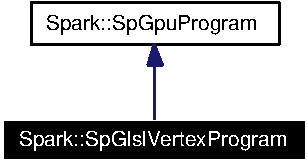
\includegraphics[width=91pt]{classSpark_1_1SpGlslVertexProgram__inherit__graph}
\end{center}
\end{figure}
Collaboration diagram for Spark::Sp\-Glsl\-Vertex\-Program:\begin{figure}[H]
\begin{center}
\leavevmode
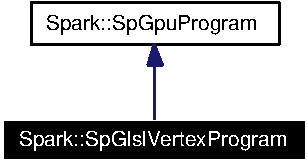
\includegraphics[width=91pt]{classSpark_1_1SpGlslVertexProgram__coll__graph}
\end{center}
\end{figure}


\subsection{Detailed Description}
Interface for a GLSL Fragment Program. 

Definition at line 32 of file Sp\-Glsl\-Vertex\-Program.h.\subsection*{Public Member Functions}
\begin{CompactItemize}
\item 
{\bf Sp\-Glsl\-Vertex\-Program} (const char $\ast$ac\-Source)
\begin{CompactList}\small\item\em Construction:. \item\end{CompactList}\item 
virtual bool {\bf set\-Parameter1i} (const char $\ast$ac\-Name, int i\-X)
\begin{CompactList}\small\item\em Access Methods:. \item\end{CompactList}\item 
virtual bool {\bf set\-Parameter2i} (const char $\ast$ac\-Name, int i\-X, int i\-Y)
\item 
virtual bool {\bf set\-Parameter3i} (const char $\ast$ac\-Name, int i\-X, int i\-Y, int i\-Z)
\item 
virtual bool {\bf set\-Parameter4i} (const char $\ast$ac\-Name, int i\-X, int i\-Y, int i\-Z, int i\-W)
\item 
virtual bool {\bf set\-Parameter1iv} (const char $\ast$ac\-Name, const int $\ast$ai\-Values, int i\-Count=1)
\item 
virtual bool {\bf set\-Parameter2iv} (const char $\ast$ac\-Name, const int $\ast$ai\-Values, int i\-Count=1)
\item 
virtual bool {\bf set\-Parameter3iv} (const char $\ast$ac\-Name, const int $\ast$ai\-Values, int i\-Count=1)
\item 
virtual bool {\bf set\-Parameter4iv} (const char $\ast$ac\-Name, const int $\ast$ai\-Values, int i\-Count=1)
\item 
virtual bool {\bf set\-Parameter1f} (const char $\ast$ac\-Name, float f\-X)
\item 
virtual bool {\bf set\-Parameter2f} (const char $\ast$ac\-Name, float f\-X, float f\-Y)
\item 
virtual bool {\bf set\-Parameter3f} (const char $\ast$ac\-Name, float f\-X, float f\-Y, float f\-Z)
\item 
virtual bool {\bf set\-Parameter4f} (const char $\ast$ac\-Name, float f\-X, float f\-Y, float f\-Z, float f\-W)
\item 
virtual bool {\bf set\-Parameter1fv} (const char $\ast$ac\-Name, const float $\ast$af\-Values, int i\-Count=1)
\item 
virtual bool {\bf set\-Parameter2fv} (const char $\ast$ac\-Name, const float $\ast$af\-Values, int i\-Count=1)
\item 
virtual bool {\bf set\-Parameter3fv} (const char $\ast$ac\-Name, const float $\ast$af\-Values, int i\-Count=1)
\item 
virtual bool {\bf set\-Parameter4fv} (const char $\ast$ac\-Name, const float $\ast$af\-Values, int i\-Count=1)
\item 
virtual bool {\bf set\-Matrix\-Parameter2fv} (const char $\ast$ac\-Name, const float $\ast$af\-Values, int i\-Count=1)
\item 
virtual bool {\bf set\-Matrix\-Parameter3fv} (const char $\ast$ac\-Name, const float $\ast$af\-Values, int i\-Count=1)
\item 
virtual bool {\bf set\-Matrix\-Parameter4fv} (const char $\ast$ac\-Name, const float $\ast$af\-Values, int i\-Count=1)
\end{CompactItemize}
\subsection*{Protected Member Functions}
\begin{CompactItemize}
\item 
{\bf Sp\-Glsl\-Vertex\-Program} ()
\begin{CompactList}\small\item\em Constructor for load function. \item\end{CompactList}\item 
int {\bf get\-Parameter\-Register} (const char $\ast$ac\-Name)
\end{CompactItemize}


\subsection{Constructor \& Destructor Documentation}
\index{Spark::SpGlslVertexProgram@{Spark::Sp\-Glsl\-Vertex\-Program}!SpGlslVertexProgram@{SpGlslVertexProgram}}
\index{SpGlslVertexProgram@{SpGlslVertexProgram}!Spark::SpGlslVertexProgram@{Spark::Sp\-Glsl\-Vertex\-Program}}
\subsubsection{\setlength{\rightskip}{0pt plus 5cm}Sp\-Glsl\-Vertex\-Program::Sp\-Glsl\-Vertex\-Program (const char $\ast$ {\em ac\-Source})}\label{classSpark_1_1SpGlslVertexProgram_a0}


Construction:. 

Definition at line 8 of file Sp\-Glsl\-Vertex\-Program.cpp.

References Spark::Sp\-Gpu\-Program::set\-Source().\index{Spark::SpGlslVertexProgram@{Spark::Sp\-Glsl\-Vertex\-Program}!SpGlslVertexProgram@{SpGlslVertexProgram}}
\index{SpGlslVertexProgram@{SpGlslVertexProgram}!Spark::SpGlslVertexProgram@{Spark::Sp\-Glsl\-Vertex\-Program}}
\subsubsection{\setlength{\rightskip}{0pt plus 5cm}Sp\-Glsl\-Vertex\-Program::Sp\-Glsl\-Vertex\-Program ()\hspace{0.3cm}{\tt  [protected]}}\label{classSpark_1_1SpGlslVertexProgram_b0}


Constructor for load function. 

Definition at line 15 of file Sp\-Glsl\-Vertex\-Program.cpp.

\subsection{Member Function Documentation}
\index{Spark::SpGlslVertexProgram@{Spark::Sp\-Glsl\-Vertex\-Program}!getParameterRegister@{getParameterRegister}}
\index{getParameterRegister@{getParameterRegister}!Spark::SpGlslVertexProgram@{Spark::Sp\-Glsl\-Vertex\-Program}}
\subsubsection{\setlength{\rightskip}{0pt plus 5cm}int Sp\-Glsl\-Vertex\-Program::get\-Parameter\-Register (const char $\ast$ {\em ac\-Name})\hspace{0.3cm}{\tt  [protected]}}\label{classSpark_1_1SpGlslVertexProgram_b1}


Definition at line 21 of file Sp\-Glsl\-Vertex\-Program.cpp.

References Spark::Sp\-Gpu\-Program::get\-User\-Data().

Referenced by set\-Matrix\-Parameter2fv(), set\-Matrix\-Parameter3fv(), set\-Matrix\-Parameter4fv(), set\-Parameter1f(), set\-Parameter1fv(), set\-Parameter1i(), set\-Parameter1iv(), set\-Parameter2f(), set\-Parameter2fv(), set\-Parameter2i(), set\-Parameter2iv(), set\-Parameter3f(), set\-Parameter3fv(), set\-Parameter3i(), set\-Parameter3iv(), set\-Parameter4f(), set\-Parameter4fv(), set\-Parameter4i(), and set\-Parameter4iv().\index{Spark::SpGlslVertexProgram@{Spark::Sp\-Glsl\-Vertex\-Program}!setMatrixParameter2fv@{setMatrixParameter2fv}}
\index{setMatrixParameter2fv@{setMatrixParameter2fv}!Spark::SpGlslVertexProgram@{Spark::Sp\-Glsl\-Vertex\-Program}}
\subsubsection{\setlength{\rightskip}{0pt plus 5cm}bool Sp\-Glsl\-Vertex\-Program::set\-Matrix\-Parameter2fv (const char $\ast$ {\em ac\-Name}, const float $\ast$ {\em af\-Values}, int {\em i\-Count} = {\tt 1})\hspace{0.3cm}{\tt  [virtual]}}\label{classSpark_1_1SpGlslVertexProgram_a17}




Reimplemented from {\bf Spark::Sp\-Gpu\-Program} {\rm (p.\,\pageref{classSpark_1_1SpGpuProgram_a28})}.

Definition at line 231 of file Sp\-Glsl\-Vertex\-Program.cpp.

References get\-Parameter\-Register().\index{Spark::SpGlslVertexProgram@{Spark::Sp\-Glsl\-Vertex\-Program}!setMatrixParameter3fv@{setMatrixParameter3fv}}
\index{setMatrixParameter3fv@{setMatrixParameter3fv}!Spark::SpGlslVertexProgram@{Spark::Sp\-Glsl\-Vertex\-Program}}
\subsubsection{\setlength{\rightskip}{0pt plus 5cm}bool Sp\-Glsl\-Vertex\-Program::set\-Matrix\-Parameter3fv (const char $\ast$ {\em ac\-Name}, const float $\ast$ {\em af\-Values}, int {\em i\-Count} = {\tt 1})\hspace{0.3cm}{\tt  [virtual]}}\label{classSpark_1_1SpGlslVertexProgram_a18}




Reimplemented from {\bf Spark::Sp\-Gpu\-Program} {\rm (p.\,\pageref{classSpark_1_1SpGpuProgram_a29})}.

Definition at line 243 of file Sp\-Glsl\-Vertex\-Program.cpp.

References get\-Parameter\-Register().\index{Spark::SpGlslVertexProgram@{Spark::Sp\-Glsl\-Vertex\-Program}!setMatrixParameter4fv@{setMatrixParameter4fv}}
\index{setMatrixParameter4fv@{setMatrixParameter4fv}!Spark::SpGlslVertexProgram@{Spark::Sp\-Glsl\-Vertex\-Program}}
\subsubsection{\setlength{\rightskip}{0pt plus 5cm}bool Sp\-Glsl\-Vertex\-Program::set\-Matrix\-Parameter4fv (const char $\ast$ {\em ac\-Name}, const float $\ast$ {\em af\-Values}, int {\em i\-Count} = {\tt 1})\hspace{0.3cm}{\tt  [virtual]}}\label{classSpark_1_1SpGlslVertexProgram_a19}




Reimplemented from {\bf Spark::Sp\-Gpu\-Program} {\rm (p.\,\pageref{classSpark_1_1SpGpuProgram_a30})}.

Definition at line 255 of file Sp\-Glsl\-Vertex\-Program.cpp.

References get\-Parameter\-Register().\index{Spark::SpGlslVertexProgram@{Spark::Sp\-Glsl\-Vertex\-Program}!setParameter1f@{setParameter1f}}
\index{setParameter1f@{setParameter1f}!Spark::SpGlslVertexProgram@{Spark::Sp\-Glsl\-Vertex\-Program}}
\subsubsection{\setlength{\rightskip}{0pt plus 5cm}bool Sp\-Glsl\-Vertex\-Program::set\-Parameter1f (const char $\ast$ {\em ac\-Name}, float {\em f\-X})\hspace{0.3cm}{\tt  [virtual]}}\label{classSpark_1_1SpGlslVertexProgram_a9}




Reimplemented from {\bf Spark::Sp\-Gpu\-Program} {\rm (p.\,\pageref{classSpark_1_1SpGpuProgram_a20})}.

Definition at line 135 of file Sp\-Glsl\-Vertex\-Program.cpp.

References get\-Parameter\-Register().

Referenced by Spark::Sp\-Vertex\-Noise\-Sb::enable().\index{Spark::SpGlslVertexProgram@{Spark::Sp\-Glsl\-Vertex\-Program}!setParameter1fv@{setParameter1fv}}
\index{setParameter1fv@{setParameter1fv}!Spark::SpGlslVertexProgram@{Spark::Sp\-Glsl\-Vertex\-Program}}
\subsubsection{\setlength{\rightskip}{0pt plus 5cm}bool Sp\-Glsl\-Vertex\-Program::set\-Parameter1fv (const char $\ast$ {\em ac\-Name}, const float $\ast$ {\em af\-Values}, int {\em i\-Count} = {\tt 1})\hspace{0.3cm}{\tt  [virtual]}}\label{classSpark_1_1SpGlslVertexProgram_a13}




Reimplemented from {\bf Spark::Sp\-Gpu\-Program} {\rm (p.\,\pageref{classSpark_1_1SpGpuProgram_a24})}.

Definition at line 183 of file Sp\-Glsl\-Vertex\-Program.cpp.

References get\-Parameter\-Register().\index{Spark::SpGlslVertexProgram@{Spark::Sp\-Glsl\-Vertex\-Program}!setParameter1i@{setParameter1i}}
\index{setParameter1i@{setParameter1i}!Spark::SpGlslVertexProgram@{Spark::Sp\-Glsl\-Vertex\-Program}}
\subsubsection{\setlength{\rightskip}{0pt plus 5cm}bool Sp\-Glsl\-Vertex\-Program::set\-Parameter1i (const char $\ast$ {\em ac\-Name}, int {\em i\-X})\hspace{0.3cm}{\tt  [virtual]}}\label{classSpark_1_1SpGlslVertexProgram_a1}


Access Methods:. 



Reimplemented from {\bf Spark::Sp\-Gpu\-Program} {\rm (p.\,\pageref{classSpark_1_1SpGpuProgram_a12})}.

Definition at line 39 of file Sp\-Glsl\-Vertex\-Program.cpp.

References get\-Parameter\-Register().\index{Spark::SpGlslVertexProgram@{Spark::Sp\-Glsl\-Vertex\-Program}!setParameter1iv@{setParameter1iv}}
\index{setParameter1iv@{setParameter1iv}!Spark::SpGlslVertexProgram@{Spark::Sp\-Glsl\-Vertex\-Program}}
\subsubsection{\setlength{\rightskip}{0pt plus 5cm}bool Sp\-Glsl\-Vertex\-Program::set\-Parameter1iv (const char $\ast$ {\em ac\-Name}, const int $\ast$ {\em ai\-Values}, int {\em i\-Count} = {\tt 1})\hspace{0.3cm}{\tt  [virtual]}}\label{classSpark_1_1SpGlslVertexProgram_a5}


Definition at line 87 of file Sp\-Glsl\-Vertex\-Program.cpp.

References get\-Parameter\-Register().\index{Spark::SpGlslVertexProgram@{Spark::Sp\-Glsl\-Vertex\-Program}!setParameter2f@{setParameter2f}}
\index{setParameter2f@{setParameter2f}!Spark::SpGlslVertexProgram@{Spark::Sp\-Glsl\-Vertex\-Program}}
\subsubsection{\setlength{\rightskip}{0pt plus 5cm}bool Sp\-Glsl\-Vertex\-Program::set\-Parameter2f (const char $\ast$ {\em ac\-Name}, float {\em f\-X}, float {\em f\-Y})\hspace{0.3cm}{\tt  [virtual]}}\label{classSpark_1_1SpGlslVertexProgram_a10}




Reimplemented from {\bf Spark::Sp\-Gpu\-Program} {\rm (p.\,\pageref{classSpark_1_1SpGpuProgram_a21})}.

Definition at line 147 of file Sp\-Glsl\-Vertex\-Program.cpp.

References get\-Parameter\-Register().\index{Spark::SpGlslVertexProgram@{Spark::Sp\-Glsl\-Vertex\-Program}!setParameter2fv@{setParameter2fv}}
\index{setParameter2fv@{setParameter2fv}!Spark::SpGlslVertexProgram@{Spark::Sp\-Glsl\-Vertex\-Program}}
\subsubsection{\setlength{\rightskip}{0pt plus 5cm}bool Sp\-Glsl\-Vertex\-Program::set\-Parameter2fv (const char $\ast$ {\em ac\-Name}, const float $\ast$ {\em af\-Values}, int {\em i\-Count} = {\tt 1})\hspace{0.3cm}{\tt  [virtual]}}\label{classSpark_1_1SpGlslVertexProgram_a14}




Reimplemented from {\bf Spark::Sp\-Gpu\-Program} {\rm (p.\,\pageref{classSpark_1_1SpGpuProgram_a25})}.

Definition at line 195 of file Sp\-Glsl\-Vertex\-Program.cpp.

References get\-Parameter\-Register().\index{Spark::SpGlslVertexProgram@{Spark::Sp\-Glsl\-Vertex\-Program}!setParameter2i@{setParameter2i}}
\index{setParameter2i@{setParameter2i}!Spark::SpGlslVertexProgram@{Spark::Sp\-Glsl\-Vertex\-Program}}
\subsubsection{\setlength{\rightskip}{0pt plus 5cm}bool Sp\-Glsl\-Vertex\-Program::set\-Parameter2i (const char $\ast$ {\em ac\-Name}, int {\em i\-X}, int {\em i\-Y})\hspace{0.3cm}{\tt  [virtual]}}\label{classSpark_1_1SpGlslVertexProgram_a2}




Reimplemented from {\bf Spark::Sp\-Gpu\-Program} {\rm (p.\,\pageref{classSpark_1_1SpGpuProgram_a13})}.

Definition at line 51 of file Sp\-Glsl\-Vertex\-Program.cpp.

References get\-Parameter\-Register().\index{Spark::SpGlslVertexProgram@{Spark::Sp\-Glsl\-Vertex\-Program}!setParameter2iv@{setParameter2iv}}
\index{setParameter2iv@{setParameter2iv}!Spark::SpGlslVertexProgram@{Spark::Sp\-Glsl\-Vertex\-Program}}
\subsubsection{\setlength{\rightskip}{0pt plus 5cm}bool Sp\-Glsl\-Vertex\-Program::set\-Parameter2iv (const char $\ast$ {\em ac\-Name}, const int $\ast$ {\em ai\-Values}, int {\em i\-Count} = {\tt 1})\hspace{0.3cm}{\tt  [virtual]}}\label{classSpark_1_1SpGlslVertexProgram_a6}


Definition at line 99 of file Sp\-Glsl\-Vertex\-Program.cpp.

References get\-Parameter\-Register().\index{Spark::SpGlslVertexProgram@{Spark::Sp\-Glsl\-Vertex\-Program}!setParameter3f@{setParameter3f}}
\index{setParameter3f@{setParameter3f}!Spark::SpGlslVertexProgram@{Spark::Sp\-Glsl\-Vertex\-Program}}
\subsubsection{\setlength{\rightskip}{0pt plus 5cm}bool Sp\-Glsl\-Vertex\-Program::set\-Parameter3f (const char $\ast$ {\em ac\-Name}, float {\em f\-X}, float {\em f\-Y}, float {\em f\-Z})\hspace{0.3cm}{\tt  [virtual]}}\label{classSpark_1_1SpGlslVertexProgram_a11}




Reimplemented from {\bf Spark::Sp\-Gpu\-Program} {\rm (p.\,\pageref{classSpark_1_1SpGpuProgram_a22})}.

Definition at line 159 of file Sp\-Glsl\-Vertex\-Program.cpp.

References get\-Parameter\-Register().\index{Spark::SpGlslVertexProgram@{Spark::Sp\-Glsl\-Vertex\-Program}!setParameter3fv@{setParameter3fv}}
\index{setParameter3fv@{setParameter3fv}!Spark::SpGlslVertexProgram@{Spark::Sp\-Glsl\-Vertex\-Program}}
\subsubsection{\setlength{\rightskip}{0pt plus 5cm}bool Sp\-Glsl\-Vertex\-Program::set\-Parameter3fv (const char $\ast$ {\em ac\-Name}, const float $\ast$ {\em af\-Values}, int {\em i\-Count} = {\tt 1})\hspace{0.3cm}{\tt  [virtual]}}\label{classSpark_1_1SpGlslVertexProgram_a15}




Reimplemented from {\bf Spark::Sp\-Gpu\-Program} {\rm (p.\,\pageref{classSpark_1_1SpGpuProgram_a26})}.

Definition at line 207 of file Sp\-Glsl\-Vertex\-Program.cpp.

References get\-Parameter\-Register().\index{Spark::SpGlslVertexProgram@{Spark::Sp\-Glsl\-Vertex\-Program}!setParameter3i@{setParameter3i}}
\index{setParameter3i@{setParameter3i}!Spark::SpGlslVertexProgram@{Spark::Sp\-Glsl\-Vertex\-Program}}
\subsubsection{\setlength{\rightskip}{0pt plus 5cm}bool Sp\-Glsl\-Vertex\-Program::set\-Parameter3i (const char $\ast$ {\em ac\-Name}, int {\em i\-X}, int {\em i\-Y}, int {\em i\-Z})\hspace{0.3cm}{\tt  [virtual]}}\label{classSpark_1_1SpGlslVertexProgram_a3}




Reimplemented from {\bf Spark::Sp\-Gpu\-Program} {\rm (p.\,\pageref{classSpark_1_1SpGpuProgram_a14})}.

Definition at line 63 of file Sp\-Glsl\-Vertex\-Program.cpp.

References get\-Parameter\-Register().\index{Spark::SpGlslVertexProgram@{Spark::Sp\-Glsl\-Vertex\-Program}!setParameter3iv@{setParameter3iv}}
\index{setParameter3iv@{setParameter3iv}!Spark::SpGlslVertexProgram@{Spark::Sp\-Glsl\-Vertex\-Program}}
\subsubsection{\setlength{\rightskip}{0pt plus 5cm}bool Sp\-Glsl\-Vertex\-Program::set\-Parameter3iv (const char $\ast$ {\em ac\-Name}, const int $\ast$ {\em ai\-Values}, int {\em i\-Count} = {\tt 1})\hspace{0.3cm}{\tt  [virtual]}}\label{classSpark_1_1SpGlslVertexProgram_a7}


Definition at line 111 of file Sp\-Glsl\-Vertex\-Program.cpp.

References get\-Parameter\-Register().\index{Spark::SpGlslVertexProgram@{Spark::Sp\-Glsl\-Vertex\-Program}!setParameter4f@{setParameter4f}}
\index{setParameter4f@{setParameter4f}!Spark::SpGlslVertexProgram@{Spark::Sp\-Glsl\-Vertex\-Program}}
\subsubsection{\setlength{\rightskip}{0pt plus 5cm}bool Sp\-Glsl\-Vertex\-Program::set\-Parameter4f (const char $\ast$ {\em ac\-Name}, float {\em f\-X}, float {\em f\-Y}, float {\em f\-Z}, float {\em f\-W})\hspace{0.3cm}{\tt  [virtual]}}\label{classSpark_1_1SpGlslVertexProgram_a12}




Reimplemented from {\bf Spark::Sp\-Gpu\-Program} {\rm (p.\,\pageref{classSpark_1_1SpGpuProgram_a23})}.

Definition at line 171 of file Sp\-Glsl\-Vertex\-Program.cpp.

References get\-Parameter\-Register().\index{Spark::SpGlslVertexProgram@{Spark::Sp\-Glsl\-Vertex\-Program}!setParameter4fv@{setParameter4fv}}
\index{setParameter4fv@{setParameter4fv}!Spark::SpGlslVertexProgram@{Spark::Sp\-Glsl\-Vertex\-Program}}
\subsubsection{\setlength{\rightskip}{0pt plus 5cm}bool Sp\-Glsl\-Vertex\-Program::set\-Parameter4fv (const char $\ast$ {\em ac\-Name}, const float $\ast$ {\em af\-Values}, int {\em i\-Count} = {\tt 1})\hspace{0.3cm}{\tt  [virtual]}}\label{classSpark_1_1SpGlslVertexProgram_a16}




Reimplemented from {\bf Spark::Sp\-Gpu\-Program} {\rm (p.\,\pageref{classSpark_1_1SpGpuProgram_a27})}.

Definition at line 219 of file Sp\-Glsl\-Vertex\-Program.cpp.

References get\-Parameter\-Register().

Referenced by Spark::Sp\-Vertex\-Noise\-Sb::initialize().\index{Spark::SpGlslVertexProgram@{Spark::Sp\-Glsl\-Vertex\-Program}!setParameter4i@{setParameter4i}}
\index{setParameter4i@{setParameter4i}!Spark::SpGlslVertexProgram@{Spark::Sp\-Glsl\-Vertex\-Program}}
\subsubsection{\setlength{\rightskip}{0pt plus 5cm}bool Sp\-Glsl\-Vertex\-Program::set\-Parameter4i (const char $\ast$ {\em ac\-Name}, int {\em i\-X}, int {\em i\-Y}, int {\em i\-Z}, int {\em i\-W})\hspace{0.3cm}{\tt  [virtual]}}\label{classSpark_1_1SpGlslVertexProgram_a4}




Reimplemented from {\bf Spark::Sp\-Gpu\-Program} {\rm (p.\,\pageref{classSpark_1_1SpGpuProgram_a15})}.

Definition at line 75 of file Sp\-Glsl\-Vertex\-Program.cpp.

References get\-Parameter\-Register().\index{Spark::SpGlslVertexProgram@{Spark::Sp\-Glsl\-Vertex\-Program}!setParameter4iv@{setParameter4iv}}
\index{setParameter4iv@{setParameter4iv}!Spark::SpGlslVertexProgram@{Spark::Sp\-Glsl\-Vertex\-Program}}
\subsubsection{\setlength{\rightskip}{0pt plus 5cm}bool Sp\-Glsl\-Vertex\-Program::set\-Parameter4iv (const char $\ast$ {\em ac\-Name}, const int $\ast$ {\em ai\-Values}, int {\em i\-Count} = {\tt 1})\hspace{0.3cm}{\tt  [virtual]}}\label{classSpark_1_1SpGlslVertexProgram_a8}


Definition at line 123 of file Sp\-Glsl\-Vertex\-Program.cpp.

References get\-Parameter\-Register().

The documentation for this class was generated from the following files:\begin{CompactItemize}
\item 
{\bf Sp\-Glsl\-Vertex\-Program.h}\item 
{\bf Sp\-Glsl\-Vertex\-Program.cpp}\end{CompactItemize}
